\documentclass[thesis.tex]{subfiles}

\begin{document}

\chapter{KdV5 with periodic boundary conditions}

\section{Background}

The 5th order KdV equation (KdV5), when written in a moving frame with speed $c$, is
\begin{equation}\label{KdV5}
u_t = \partial_x(u_{xxxx} - u_{xx} - u^2 + cu) 
\end{equation}
We can write this as $u_t = \partial_x E'(u)$, where $E(u)$ is the energy
\begin{equation}\label{energy}
E(u) = -\int_{-\infty}^{\infty} \left( \frac{1}{2}u_{xx}^2 + \frac{1}{2}u_x^2 + \frac{1}{2}cu^2 - \frac{1}{3}u^3 \right) dx
\end{equation}
The energy $E(u)$ is conserved (in $t$) and is translation invariant. In addition, $E'(u)$ is reversible; in particular, this means that the linear part of $E'(u)$ only involves even order derivatives.

An equilibrium solution to \eqref{KdV5} satisfies the 5th order nonlinear ODE
\begin{equation}\label{eqODE}
u_{xxxxx} - u_{xxx} + c u_x - 2 u u_x = 0
\end{equation}
The rest state $u = 0$ is a solution to \eqref{eqODE}. A primary pulse solution is a homoclinic orbit which connects the rest state to itself. A primary pulse solution must also satisfy the 4th order ODE
\begin{equation}\label{eqODE4}
u_{xxxx} - u_{xx} + c u - u^2 = 0,
\end{equation}
which is obtained from \eqref{eqODE} by integrating once; we can take the constant of integration to be 0 since we are seeking a solution which decays to the rest state. Equation \eqref{eqODE4} is Hamiltonian, with energy given by
\begin{equation}\label{Hamiltonian}
H(u, u', u'', u''') = u'u''' - \frac{1}{2}(u'^2) - \frac{1}{2}(u'')^2 + \frac{c}{2}u^2 - \frac{1}{3}u^3 
\end{equation}
The Hamiltonian $H$ is conserved (in $x$). We can write this in standard form by taking
\[
Q = (q_1, q_2, p_1, p_2) = (u, u', -u''' + u', u'')
\]
in which case we have $Q' = J \nabla \tilde{H} Q$, where
\begin{equation}
H(q_1, q_2, p_1, p_2) = \frac{1}{3}q_1^3 - \frac{1}{2}c q_1^2 + p_1 q_1 - \frac{1}{2}q_2^2 + \frac{1}{2}p_2^2
\end{equation}
and $J$ is standard $4 \timed 4$ symplectic matrix.

The linearization of the 4th order ODE \eqref{eqODE4} about a solution $u^*(x)$ of \eqref{eqODE4} is the self-adjoint linear operator
\begin{equation}\label{defA0}
A_0(u^*) = E''(u^*) = \partial_x^4 - \partial_x^2 + c - 2 u^* 
\end{equation}
The eigenvalues of the linearization about the rest state $u^* = 0$ are the solutions to the fourth-order polynomial equation $\nu^4 - \nu^2 + c = 0$, which are
\begin{align}\label{specA0}
\nu = \pm \sqrt{ \frac{1 \pm \sqrt{1 - 4c} }{2}}
\end{align}
Since two eigenvalues have positive real part and two have negative real part, the equilibrium at 0 is hyperbolic with a two-dimensional stable manifold and a two-dimensional unstable manifold. For $0 < c < 1/4$, all four eigenvalues are real. A bifurcation takes place at $c = 1/4$, and for $c > 1/4$, there is a quartet of eigenvalues of the form $\pm \alpha_0 \pm \beta_0 i$, where $\alpha_0, \beta_0 > 0$.

For $c > 0$, a symmetric homoclinic orbit solution $q(x)$ exists to \eqref{eqODE4} \cite[Theorem 2.1]{Pelinovsky2007}. For $c > 1/4$. the existence of multi-pulse homoclinic orbits follows from \cite{SandstedeStrut}. We are interested in periodic, multi-pulse solutions.

\section{General Setup}

We will write the problem in general terms, for which KdV5 will be a specific case. Consider the PDE
\begin{equation}\label{genPDE}
u_t = \partial_x E'(u)
\end{equation}
where $u \in H^{2m}(\R)$ and $E'(u): H^{2m}(\R) \subset L^2(\R) \rightarrow L^2(\R)$. $E(u)$ is the energy of the system (which is conserved in $t$), and $E(0) = 0$. We take the following hypothesis regarding $E'(u)$.

\begin{hypothesis}\label{Eprimehyp}
The operator $E'(u)$ has the following properties
\begin{enumerate}[(i)]
\item $E'(u)$ is of the form
\begin{equation}\label{Eprimeuform}
E'(u) = \partial_x^{2m}u + \tilde{E}(u)
\end{equation}
where all derivatives involved in $\tilde{E}(u)$ are order $2m-1$ and lower.
\item $E'(u)$ is reversible, i.e. $E'(u) = 0$ implies $E'(\rho(u)) = 0$,
where $[\rho(u)](x) = u(-x)$.
\item $E'(u)$ is translation invariant, i.e. $E'(u) = 0$ implies $E'(\tau_\xi(u)) = 0$ for all $\xi \in \R$, where $[\tau_\xi(u)](x) = u(x - \xi)$.
\end{enumerate}
\end{hypothesis}
Reversibility implies that the linear part of the operator $E'(u)$ only involves even-order derivatives of $u$ with respect to $x$. If $u(x)$ is an even function, the nonlinear part is also an even function in $x$.

Equilibrium solutions which decay to 0 at $\pm \infty$ satisfy the ODE 
\begin{equation}\label{ODEonR}
E'(u) = \partial_x^{2m}u + \tilde{E}(u) = 0
\end{equation}
which is obtained from \eqref{genPDE} by taking $u_t = 0$ and integrating once. By Hypothesis \ref{Eprimehyp}, the highest order derivative $\partial_x^{2m}$ in $E'(u)$ appears by itself with a coefficient of 1. Thus we can write \eqref{ODEonR} as a first-order system in the standard way as
\begin{equation}\label{genODE}
U'(x) = F(U(x))
\end{equation}
where $U = (u, \partial_x u, \dots, \partial_x^{2m-1} u) \in \R^{2m}$, $F: \R^{2m} \rightarrow \R^{2m}$ is smooth, and $F(0) = 0$. The reversibility hypothesis implies that
\begin{equation}\label{genODErev}
F(RU) = -RF(U)
\end{equation}
where $R:\R^{2m} \rightarrow \R^{2m}$ is the standard reversor operator defined by
\begin{equation}\label{reverserR2m}
R(u_1, u_2, \dots, u_{2m-1}, u_{2m}) = (u_1, -u_2, \dots, u_{2m-1}, -u_{2m})
\end{equation}
In particular, if $U(x)$ is a solution to \eqref{genODE}, so is $RU(-x)$.

First, we will prove that periodic multi-pulse solutions exist. We will then study their spectral stability.

\section{Existence of Periodic Multi-pulses}

An $n-$periodic solution to \eqref{genODE} is a periodic orbit which resembles $n$ well-separated copies of the primary pulse. The $n$ peaks are separated by distances $2X_0, 2X_1, \dots, 2X_{n-1}$, as shown in Figure \ref{fig:permultipulse}.

\begin{figure}[H]
\label{fig:permultipulse}
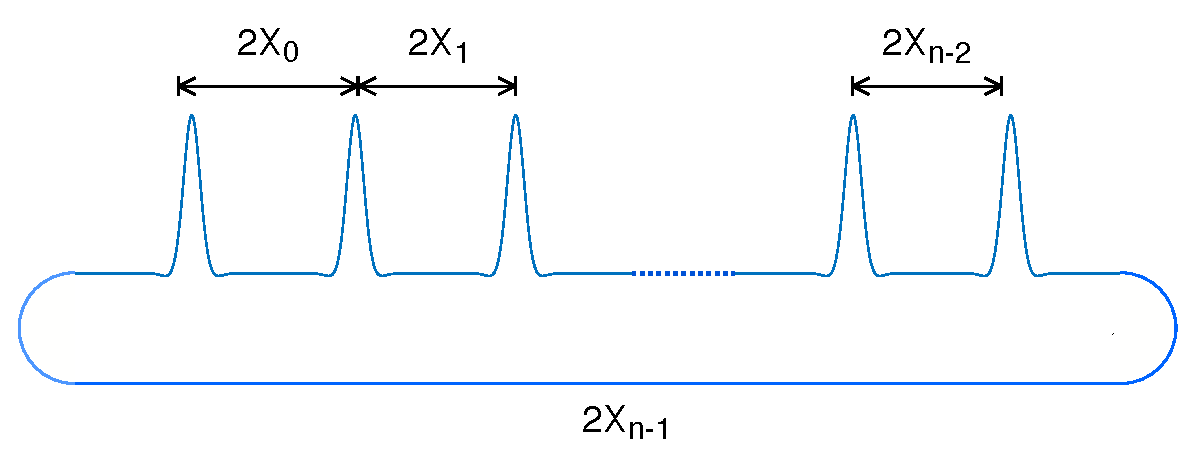
\includegraphics[width=10cm]{periodic/multipulseperiodic}
\caption{Periodic $n-$pulse solution.}
\end{figure} 

In order to prove the existence of such solutions, we take the following hypotheses. First, we assume that equation \eqref{genODE} is Hamiltonian.
\begin{hypothesis}\label{Hhyp}
There exists a smooth function $H: \R^{2m} \rightarrow \R$ such that 
\begin{enumerate}[(i)]
\item $H(0) = 0$
\item $\nabla H(u) = 0$ if and only if $F(u) = 0$
\item For all $u \in \R^{2m}$,
\begin{equation}
\langle \nabla H(u), F(u) \rangle = 0
\end{equation}
\end{enumerate}
\end{hypothesis}
It follows from this hypothesis that $H$ is conserved along solutions $U(x)$ to \eqref{genODE}. The next hypothesis addresses the hyperbolicity of the equilibrium of \eqref{genODE} at $U = 0$.  
\begin{hypothesis}\label{hypeqhyp}
$U = 0$ is a hyperbolic equilibrium of \eqref{genODE}, i.e. $DF(0)$ has no eigenvalues on the imaginary axis. Furthermore, the spectrum of $DF(0)$ contains a quartet of simple eigenvalues $\pm \alpha_0 \pm \beta_0 i$, $\alpha_0, \beta_0 > 0$, and for any other eigenvalue $\nu$ of $DF(0)$, $|\text{Re }\nu| > \alpha_0$.
\end{hypothesis}
We remark that since we have a Hamiltonian system, the existence of an eigenvalue $\alpha_0 + \beta_0 i$ of $DF(0)$ implies the existence of the entire quartet $\pm \alpha_0 \pm \beta_0 i$. Let $E_0^s$ and $E_0^u$ be the stable and unstable eigenspaces of $DF(0)$. By reversibility, both of these spaces have dimension $m$.

Let $W^s(0)$ and $W^u(0)$ be the stable and unstable manifolds of the equilibrium at 0. By Hypothesis \ref{Hhyp}, $W^s(0), W^u(0) \subset H^{-1}(0)$, where $H^{-1}(0)$ is the 0-level set of $H$. By reversibility, $\dim W^s(0) = m$ and $\dim W^u(0) = m$. 

In the next hypothesis, we assume that a symmetric homoclinic orbit solution exists to \eqref{genODE}.
\begin{hypothesis}\label{Qexistshyp}
A homoclinic orbit solution $Q(x) \in W^s(0) \cap W^u(0) \subset H^{-1}(0)$ exists to \eqref{genODE}. Furthermore, this solution is symmetric with respect to the reversor operator \eqref{reverserR2m}, i.e. $Q(-x) = R Q(x)$.
\end{hypothesis}
 
Since we obtained \eqref{genODE} by putting \eqref{ODEonR} into a first order system in the standard way, $Q(x) = (q(x), q'(x), \dots, q^{(2m)}(x))^T$, where $q(x)$ is an even function and is an exponentially localized solution to \eqref{ODEonR}. Since $Q(x) \subset W^s(0) \cap W^u(0)$, $Q'(x) \in T_{Q(x)}W^s(0) \cap T_{Q(x)}W^u(0)$. In the next hypothesis, we take this intersection to be one-dimensional, which is a standard nondegeneracy condition.

\begin{hypothesis}\label{nondegenhyp}
Let $Q(x)$ be a symmetric homoclinic orbit solution as in Hypothesis \ref{Qexistshyp}. We take the non-degeneracy condition
\begin{equation}
T_{Q(0)}W^s(0) \cap T_{Q(0)}W^u(0) = \R Q'(0)
\end{equation}
\end{hypothesis}

The variational and adjoint variational equations associated with equation \eqref{genODE} are
\begin{align}
V' = DF(Q(x)) V \label{vareq1} \\
W' = -DF(Q(x))^* W \label{adjvareq1}
\end{align}
where $DF(Q(x))$ has the form
\begin{equation}\label{DF}
DF(Q(x)) = \begin{pmatrix}
0 & 1 & 0 & \dots & 0 & 0 \\
0 & 0 & 1 & \dots & 0 & 0 \\
& &  & \ddots &  & & \\
0 & 0 & 0 & \dots & 0 & 1 \\
c_0 + f_0(x) & f_1(x) & c_2 + f_2(x) &
 \dots & c_{2m-2} + f_{2m-2}(x) & f_{2m-1}(x)
\end{pmatrix}
\end{equation}
The variational equation \eqref{vareq1} comes from writing the linear ODE $E''(q(x))v(x) = 0$ as a first order system in the standard way, where $E''(q(x))$ is the Hessian of the energy. The constants $c_i$ come from the linear part of $E'(u)$ and do not depend on $Q(x)$. By reversibility, no odd-order derivatives are involved in the linear part of $E'(u)$, and so $c_i = 0$ for $i$ odd. In addition, since $q(x)$ is an even function, $f_i(x)$ is an even function for $i$ even and an odd function for $i$ odd. Finally, since the functions $f_i(x)$ are smooth functions of $q(x)$ and its derivatives, they decay exponentially to 0 since $q(x)$ is exponentially localized.

We make one additional assumption on the constant $c_0$, which we will need for the stability problem.
\begin{hypothesis}\label{c0nonzero}
For the constant $c_0$ in $DF(Q(x))$, $c_0 \neq 0$.
\end{hypothesis}
This hypothesis is satisfied, for example, if \eqref{genPDE} is obtained from putting a nonlinear, dispersive PDE such as KdV5 into a moving reference frame with speed $c$.

It follows from Hypothesis \ref{nondegenhyp} that $Q'(x)$ is the unique bounded solution to \eqref{vareq1}, and that there exists a unique bounded solution $\Psi(x)$ to \eqref{adjvareq1}. Since we have a Hamiltonian system, we know the exact form of $\Psi(x)$, which is given in the following lemma.

\begin{lemma}\label{psiform}
Let $H$ be the Hamiltonian from Hypothesis \ref{Hhyp}. Then $\Psi(x) = \nabla H(Q(x))$.
\end{lemma}

The next lemma gives a few important results about variational and adjoint variational equations.

\begin{lemma}\label{eigadjoint}
Consider the linear ODE $V' = A(x)V$ and the corresponding adjoint equation $W' = -A(x)^* W$, where $A$ is an $n \times n$ matrix depending on $x$. Then the following are true.
\begin{enumerate}[(i)]
\item $\dfrac{d}{dx}\langle V(x), W(x) \rangle = 0$, thus the inner product is constant in $x$.
\item If $W(x)$ is bounded and $V(x) \rightarrow 0$ as $x \rightarrow \infty$ or $V(x) \rightarrow -\infty$, then $\langle V(x), W(x) \rangle = 0$ for all $x \in \R$. The same holds if we reverse the roles of $W$ and $V$.
\item If $\Phi(y, x)$ is the evolution operator for $V'(x) = A(x)V(x)$, then $\Phi(x, y)^*$ is the evolution operator for the adjoint problem $W'(y) = -A(y)^* W(y)$.
\end{enumerate}
\end{lemma}

Next, we decompose the tangent spaces of the stable and unstable manifolds at $Q(0)$. By Hypothesis \ref{nondegenhyp}, the two tangent spaces have a one-dimensional intersection spanned by $Q'(0)$, so we can write
\begin{align*}
T_{Q(0)}W^u(0) &= \R Q'(0) \oplus Y^- \\
T_{Q(0)}W^s(0) &= \R Q'(0) \oplus Y^+
\end{align*}
From Lemma \ref{eigadjoint}(ii), $\Psi(0) \perp \R Q'(0) \oplus Y^+ \oplus Y^-$, thus we have the decomposition
\begin{equation}\label{R2mdecomp}
\R^{2m} = \R Q'(0) \oplus Y^+ \oplus Y^- \oplus Z
\end{equation}
where $Z = \R \Psi(0)$.
 
We now write $W^u(0)$ and $W^s(0)$ as graphs over their tangent spaces near $Q(0)$. Following \cite{Sandstede1997}, we can parameterize the unstable and stable manifolds near $Q(0)$ by the smooth functions $Q^-(\alpha, \beta^-)$ and $Q^+(\alpha, \beta^+)$, where $\alpha \in \R$, $\beta^\pm \in Y^\pm$ and these functions are chosen so that $Q^+(\alpha, 0) - Q^-(\alpha, 0) \in Z$. Note that $Q^+(0, 0) = Q^-(0, 0) = Q(0)$. We will always take $\alpha = 0$. Using this parameterization, let
\begin{align*}
Q^-(x; \beta^-) && x \leq 0 \\
Q^+(x; \beta^-) && x \geq 0
\end{align*}
be the unique solutions to \eqref{genODE} on $\R^\pm$ with initial conditions $Q^\pm(0, \beta^\pm)$ at $x = 0$. Since these initial conditions are on the unstable and stable manifolds (respectively), these solutions decay exponentially (in the appropriate direction) with rate $\alpha_0$.

Let $n$ be the number of pulses in the periodic solution we would like to construct. Then we will look for a solution $U$ to \eqref{genODE} which is piecewise of the form
\begin{equation}\label{Upiecewise}
\begin{aligned}
U_i^-(x) &= Q^-(x; \beta_i^-) + V_i^-(x) && x \in [-X_{i-1}, 0] \\
U_i^+(x) &= Q^+(x; \beta_i^+) + V_i^+(x) && x \in [0, X_i]
\end{aligned}
\end{equation}
where $i = 0, \dots, n-1$ and the subscripts $i$ are taken $\mod n$ since we are on a perioidic domain. Essentially, we are writing $U$ in terms of $2n$ parameters $\beta_i^\pm$, representing initial conditions on the unstable and stable manifolds, and the $2n$ remainder functions $V_i^\pm(x)$. Since the initial conditions of $Q^\pm(x; \beta_i^\pm)$ are in $\R Q'(0) \oplus Y^\pm$, we can choose $V_i^\pm(x)$ with initial conditions
\begin{align*}
V_i^-(0) &\in Z \oplus Y^- \\
V_i^+(0) &\in Z \oplus Y^+
\end{align*}

Since we are looking for a continuous solution, we need the functions $U_i^\pm(x)$ to match at each of the $2n$ boundaries between intervals. Thus, to obtain a periodic multi-pulse, we need to solve the following system of equations equations
\begin{align}
(U_i^\pm)' - F(U_i^\pm) &= 0 \label{exsystem1} \\
U_i^+(X_i) - U_{i+1}^-(-X_i) &= 0 \label{exsystem2} \\
U_i^+(0) - U_i^-(0) &= 0 \label{exsystem3}
\end{align}
where $i = 0, \dots, n-1$. To do this, we will use Lin's method. Briefly, we will show that we can find a unique piecewise solution $U_i^\pm$ satisfying \eqref{exsystem1} and \eqref{exsystem2}. This solution will have $n$ jumps at $x = 0$, which must be in the direction of $\Psi(0)$. We will derive expressions for these jumps. A periodic multipulse solution exists if and only if these $n$ jumps are all 0.

We can now state the existence theorem for periodic multi-pulse solutions. Rather than specify these solutions in terms of the lengths $X_i$, we will adopt a convenient parameterization with a built-in scaling parameter. Define the two sets
\begin{align}
\mathcal{R} &= \left\{ \exp\left(-\frac{m \pi}{\rho}\right) : m \in \N_0 \right\} \cup \{ 0 \}  \\
\mathcal{B} &= \left\{ \exp\left(-\frac{m \pi}{\rho}\right) : m \in \N_0 \right\} \label{setB}
\end{align}
where $\rho = \beta_0 / \alpha_0$. We note that $\mathcal{R}$ is a complete metric space. Then we will describe a periodic multi-pulse using the following four sets of parameters. 

\begin{enumerate}[(i)]
\item A integer $n \geq 2$, which is the number of pulses.
\item A scaling parameter $r \in \mathcal{R}$.
\item A sequence of $n$ baseline length parameters $\{ b_0^0, \dots, b_{n-1}^0 \}$, where $b_j^0 \in \mathcal{B}$.
\item A phase parameter $\theta \in [-\arctan \rho, \pi - \arctan \rho)$.
\end{enumerate}
The pulse distances $X_i$ are be determined by these parameters. We prove the existence of periodic multi-pulse solutions to \eqref{genODE} in the following theorem. The existence result requires that the scaling parameter $r$ be sufficiently small, which means that the individual pulses must be well-separated.

\begin{theorem}[Existence of $n$-periodic solutions]\label{perexist}
Assume Hypotheses \ref{Eprimehyp}, \ref{Hhyp}, \ref{hypeqhyp}, \ref{Qexistshyp}, and \ref{nondegenhyp}. Let $Q(x)$ be a transversely constructed, symmetric primary pulse solution to \eqref{genODE}. Choose
\begin{itemize}
\item An integer $n \geq 2$ 
\item A sequence of $n$ baseline length parameters $\{ b_0^0, \dots, b_{n-1}^0 \}$, where $b_j^0 = \exp\left(-\frac{m_j \pi}{\rho}\right) \in \mathcal{B}$ and at least one of the $b_j^0$ is 1. Without loss of generality, take $b_{n-1}^0 \leq b_j^0$ (equivalently, $m_{n-1} \geq m_j$) for $j = 0, \dots, n-2$.
\item A phase parameter $\theta \in [-\arctan \rho, \pi - \arctan \rho)$.
\end{itemize}
with the restriction that for $j = 0, \dots, n-2$, neither of the following is true.
\begin{itemize}
\item $m_j = m_{n-1}$ and $\theta = -\arctan \rho$
\item $m_j = m_{n-1} - 1$ and $\theta = \pi-\arctan \rho$
\end{itemize}
Then there exists $r_0 > 0$ such that
\begin{enumerate}[(i)]

\item For any $r \in \mathcal{R}$ with $r < r_0$, there exists a unique $n$-periodic solution $U(x)$ to \eqref{genODE}. Bounds for the piecewise formulation \eqref{Upiecewise} are given in Lemma \ref{solvewithjumps}.

\item This solution is specified by the $n$ length parameters $b_j(r; m_j, \theta)$, where
\begin{align}
b_j(r; m_j, \theta) \rightarrow b^*_j(m_j, \theta) \text{ as } r \rightarrow 0
\end{align}
and
\begin{align}
b^*_j(m_j, 0) = b_j^0
\end{align}
Details on this parameterization are given in Lemma \ref{thetaparamlemma}

\item The individual pulses in $U(x)$ are separated by distances $2 X_0, \dots, 2 X_{n-1}$, where 
\begin{equation}\label{Xj}
X_j = -\frac{1}{2\alpha}\log(b_j(r; m_j, \theta) r) - \frac{\phi}{2 \beta} 
\end{equation}
where $\phi$ is a constant.

\item The domain has length $2X$, where $X = X_0 + \dots + X_{n-1}$ and is given by
\begin{align}
X = \frac{1}{2\alpha} (n |\log r| + |\log b| ) - \frac{n \phi}{2 \beta}
\end{align}
where 
\begin{equation}\
b = \prod_{j=0}^{n-1} b_j(r; m_j, \theta)
\end{equation}
\end{enumerate}
\end{theorem}

If one of the baseline length parameters $b_j^0$ is small (i.e. one of the distances $X_j$ is large), the periodic $n-$pulse ``resembles'' the $n-$pulse on the real line. Without loss of generality, since we are on a periodic domain, we will choose $b_{n-1}^0$ to be small. In the next theorem, we will prove a uniform existence result. To do this, we will choose only the first $n-1$ baseline length parameters; we will allow the final baseline length parameter and the phase parameter to vary. 

\begin{theorem}\label{unifperexist}
Assume Hypotheses \ref{Eprimehyp}, \ref{Hhyp}, \ref{hypeqhyp}, \ref{Qexistshyp}, and \ref{nondegenhyp}. Let $Q(x)$ be a transversely constructed, symmetric primary pulse solution to \eqref{genODE}. Choose
\begin{itemize}
\item An integer $n \geq 2$ 
\item A sequence of $n-1$ baseline length parameters $b_0^0, \dots, b_{n-2}^0$, where $b_j^0 \in \mathcal{B}$ and at least one of the $b_j^0$ is 1.
\end{itemize}
Then there exists $r_1 > 0$ and $b^* \in \mathcal{B}$ such that for any $r < r_1$, $b_{n-1}^0 \in \mathcal{B}$ with $b_{n-1}^0 \leq b^*$, and $\theta \in [-\arctan \rho, \pi - \arctan \rho)$, there exists a unique $n$-periodic solution $U(x)$ to \eqref{genODE}. This solution is the same as the one from Theorem \ref{perexist}.
\end{theorem}

Finally, we show that for the the family of $2-$periodic pulse, there is a pitchfork bifurcation in which solutions with unequal pulse distances bifurcate off of solutions with equal pulse distances. Note that in this case we adopt a different parameterization.

\begin{theorem}\label{2pulsebifurcation}
Assume Hypotheses \ref{Eprimehyp}, \ref{Hhyp}, \ref{hypeqhyp}, \ref{Qexistshyp}, and \ref{nondegenhyp}. Let $Q(x)$ be a transversely constructed, symmetric primary pulse solution to \eqref{genODE}. For every $M \in \N$ there exists $r_0 > 0$ such that for every $r \in \mathcal{R}$ with $r < r_0$, the following is true.
\begin{enumerate}[(i)]
	\item For every $\theta \in [0, \pi)$, there is a unique 2-periodic solution with equal length parameters 
	\[
	b_0(\theta) = b_1(\theta) = e^{-\frac{1}{\rho}\theta}
	\]
	\item For every $s \in [0, M]$, there is a unique 2-periodic solution with unequal length parameters
	\[
	(\tilde{b}_0, \tilde{b}_1) = (\tilde{b}_0(s, r), \tilde{b}_1(s, r))
	\]
	where
	\[
	\tilde{b}_1(s, 0) = e^{-\frac{1}{\rho}(\arctan \rho + s)}
	\]
	and
	\[
	\tilde{b}_0(s, 0) \rightarrow 1 \text{ as } s \rightarrow \infty
	\]
	\item These two branches meet at a pitchfork bifurcation at $(p_0(r), p_0(r))$, where $p_0(r) = e^{-\frac{1}{\rho}\theta_p(r)}$ and $\theta_p(r) \rightarrow \arctan \rho$ as $r \rightarrow 0$. In terms of the two parameterizations,
	\[
	(\tilde{b}_0(0, r), \tilde{b}_1(0, r)) = (b_0(p_0(r)), b_1(p_0(r)) 
	= (p_0(r), p_0(r))
	\]
\end{enumerate}
\end{theorem}

\section{Stability}

In the previous section, we have proven existence of periodic multi-pulse solutions to \eqref{genODE}, which yield equilibrium solutions to \eqref{genPDE}. We will now look at their spectral stability. This involves finding the eigenvalues of \eqref{genPDE}. Let $u^*(x)$ be any exponentially localized equilibrium solution to \eqref{genPDE}. Substituting the standard linearization ansatz 
\[
u(x, t) = u^*(x) + \epsilon e^{\lambda t}v(x)
\]
into \eqref{genPDE} and keeping terms up to order $\epsilon$, we obtain the PDE eigenvalue problem
\begin{equation}\label{PDEeig}
\partial_x E''(u^*(x)) v = \lambda v
\end{equation}
where $E''(u^*(x))$ is the Hessian of the energy, which is self-adjoint. From the previous section, $[\partial_x E''(u^*(x))] \partial_x u^*(x) = 0$. Let $U^*(x) = (u^*(x), \partial_x u^*(x), \dots, \partial_x^{2m}u^*(x))$. Then we can write \eqref{PDEeig} as the first order system in the standard way as
\begin{equation}\label{PDEeig2}
V'(x) = A(U^*(x))V(x) + \lambda B V(x)
\end{equation}
where $A(U^*(x))$ has the same form as \eqref{DefA} below, and $B$ is the $(2m+1) \times (2m+1)$ constant coefficient matrix
\begin{equation}\label{DefB}
B = \begin{pmatrix}0 & 0 & 0 & 0 & 0 \\0 & 0 & 0 & 0 & 0 \\  & 
\vdots & & \vdots & \\0 & 0 & 0 & 0 & 0 \\1 & 0 & 0 & 0 & 0 \end{pmatrix} 
\end{equation}
Since $u^*(x)$ is exponentially localized, $A(U^*(x))$ is exponentially asymptotic to the constant coeffient matrix $A(0)$. The following lemma describes the eigenvalues of $A(0)$.

\begin{lemma}\label{eigA0lemma}
$A(0)$ has a simple eigenvalue at 0 and a quartet of eigenvalues at $\pm \alpha_0 \pm \beta_0 i$. For any other eigenvalue $\nu$ of $A(0)$, $|\text{Re }\nu| > \alpha_0$. 
\end{lemma}

Since $A(0)$ is not hyperbolic, the results of \cite{Sandstede1998} do not apply. Let $W^s(0)$, $W^u(0)$, and $W^c(0)$ be the stable, unstable, and center manifolds of the equilibrium at 0. By reversibility from Hypothesis \ref{Eprimehyp}, $\dim W^s(0) = m$ and $\dim W^u(0) = m$. The center manifold $W^c(0)$ is one-dimensional.

Let $Q(x) = (q(x), \partial_x q(x), \dots, \partial_x^{2m} q(x))$, where $q(x)$ is the symmetric primary pulse solution from Hypothesis \ref{Qexistshyp}. (We note that $Q(x) \in \R^{2m+1}$ here, so it has one additional component compared to $Q(x)$ in the previous section; for convenience, we keep the same notation since it represents the same equilibrium solution $q(x)$ to \eqref{genPDE}). The variational and adjoint variational equations associated with \eqref{PDEeig2} are
\begin{align}
V'(x) = A(Q(x)) V(x) \label{vareq2} \\
W'(x) = -A(Q(x))^* W(x) \label{adjvareq2}
\end{align}
where $A(Q(x))$ is given by
\begin{equation}\label{DefA}
A(Q(x)) = \begin{pmatrix}
0 & 1 & \dots & 0 & 0 \\
0 & 0 & \dots & 0 & 0 \\
& & \ddots  \\
0 & 0 & \dots & 0 & 1 \\
f_0'(x) & c_0 + f_0(x) + f_1'(x) & \dots & c_{2m-2} + f_{2m-2}(x) + f_{2m-1}' (x) & f_{2m-1}(x)
\end{pmatrix}
\end{equation}
where the $c_i$ and $f_i$ are the same as in \eqref{DF}. $Q'(x)$ is an exponentially localized solution to \eqref{vareq2}. Since $q(x)$ is symmetric, satisfies the reversibility property
\begin{equation}\label{vareqrev2}
A(Q(-x))RV = -RA(Q(x))V
\end{equation}

Since $Q(x)$ is exponentially localized, it cannot involve the center manifold $W^c(0)$, thus it must lie in the intersection of the stable and unstable manifolds. In particular, this implies that $\R Q'(0) \subset T_{Q(0)}W^s(0) \cap T_{Q(0)}W^u(0)$. From Hypothesis \ref{nondegenhyp}, these are actually equal, which we state in the following lemma.

\begin{lemma}\label{nondegenlemma}
We have the nondegeneracy condition
\begin{equation}\label{nondegen2}
T_{Q(0)}W^s(0) \cap T_{Q(0)}W^u(0) = \R Q'(0)
\end{equation}
\end{lemma}

Using the nondegeneracy condition \eqref{nondegen2}, we can decompose the tangent spaces of the stable and unstable manifolds at $Q(0)$ as
\begin{align*}
T_{Q(0)}W^s(0) &= \R Q'(0) \oplus Y^+ \\
T_{Q(0)}W^u(0) &= \R Q'(0) \oplus Y^- \\
\end{align*}
Since $\dim \R Q'(0) \oplus Y^+ \oplus Y^- = 2m-1$, we are missing two directions to span $\R^{2m+1}$. To find these, let $V_0$ and $W_0$ be  eigenvectors of $A(0)$ and $-A^*(0)$ corresponding to the eigenvalue 0. From \eqref{DefA}, we can choose
\begin{align}
V_0 &= (-1/c_0, 0, 0, \dots, 0)^T \label{V0} \\
W_0 &= (-c_0, 0, -c_2, 0, -c_4, 0, \dots, 0, -c_{2m-2}, 0, 1)^T \label{W0}
\end{align}
where we have scaled $V_0$ so that $\langle V_0, W_0 \rangle = 1$. We have the following lemma regarding solutions to \eqref{vareq2} and \eqref{adjvareq2}.

\begin{lemma}\label{varadjsolutions}
We have the following solutions to the variational equation \eqref{vareq2} and adjoint variational equation \eqref{adjvareq2}.
\begin{enumerate}[(i)]
\item There exists exactly two linearly independent, bounded solutions $\Psi(x)$ and $\Psi^c(x)$ to \eqref{adjvareq2}. $\Psi(x)$ is exponentially localized, i.e. $e^{\alpha |x|}\Psi(x)$ is bounded, and the last component of $\Psi(x)$ is $q(x)$. In addition, $\Psi(x)$ is symmetric with respect to the standard reversor operator $R$, i.e. $\Psi(-x) = R \Psi(x)$. The last component of $\Psi^c(x)$ is $1$, and
	\begin{equation}
	\Psi^c(x) \rightarrow W_0 \text{ as }|x| \rightarrow \infty
	\end{equation}
In addition, $\Psi(0), \Psi^c(0) \perp \R Q'(0) \oplus Y^+ \oplus Y^-$.
\item There exists a bounded solution $V^c(x)$ of \eqref{vareq2} such that 
\begin{equation}
V^c(x) \rightarrow V_0 \text{ as }|x| \rightarrow \infty
\end{equation}
Furthermore $V^c$ is symmetric with respect to the standard reversor operator $R$, i.e. $V^c(-x) = R V^c(x)$.
\end{enumerate}
\end{lemma}

Using Lemma \ref{nondegenlemma} and Lemma \ref{varadjsolutions}, we can decompose $\R^{2m+1}$ as  
\begin{equation}
\R^{2m+1} = \R \Psi(0) \oplus \R \Psi^c(0) \oplus \R Q'(0) \oplus Y^+ \oplus Y^-
\end{equation}
where $\R \Psi(0) \oplus \R \Psi^c(0) \perp \R Q'(0) \oplus Y^+ \oplus Y^-$.

Finally, we will look at the Melnikov integrals relevant to the problem. The lowest order Melnikov integral is
\begin{equation}\label{M1}
M_1 = \int_{-\infty}^\infty \langle \Psi(x), B Q'(x) \rangle =
\int_{-\infty}^\infty q(x) \: \partial_x q(x) = 0
\end{equation}
since $q(x)$ is an even function and the last component of $\Psi(x)$ is $q(x)$ by Lemma \ref{varadjsolutions}. Since $\ker [\partial_x E''(q)]^* = \ker(-E''(q) \partial_x)$, $\{ q, 1 \} \subset \ker [\partial_x E''(q)]^*$. By Lemma \ref{varadjsolutions}(i), $\ker [\partial_x E''(q)]^* = \text{span}\{ q, 1 \}$ and $q \perp \ker [\partial_x E''(q)]^*$ since both $\langle \partial_x q, q \rangle = 0$ and $\langle \partial_x q, 1 \rangle = 0$. Thus, by the Fredholm alternative, there exists a function $t(x) \in H^{2m}(\R)$ such that $[ \partial_x E''(q) ]t(x) = \partial_x q(x)$. Let $T(x) = (t(x), \partial_x t(x), \dots, \partial_x^{2m}(x))^T$. Then $T(x)$ solves the equation
\begin{equation}\label{eqforT}
T'(x) = A(Q(x))T(x) + B Q'(x)
\end{equation}

We take the following hypothesis regarding the higher order Melnikov integral.
\begin{hypothesis}\label{Melnikov2hyp}
We have the following Melnikov-like expression
\begin{equation}\label{M2}
M_2 = \int_{-\infty}^\infty \langle \Psi(x), B T(x) \rangle dx =
\int_{-\infty}^\infty q(x) t(x) dx \neq 0
\end{equation}
\end{hypothesis}

Let $q_{np}(x)$ be a periodic $n-$pulse solution constructed according to Theorem \ref{perexist}. By a similar analysis, $\partial_x E''(q_{np}) (\partial_x q_{np}(x)) = 0$, thus there exists a function $t_{np}(x) \in H^{2m}(\R)$ such that 
\begin{align*}
\partial_x E''(q_{np}) t_{np}(x) &= q_{np}(x) \\
\end{align*}

We are interested in the eigenvalues of \eqref{PDEeig} for the equilibrium solution $q_{np}(x)$. To do this, we use Lin's method to construct an eigenfunction $V(x)$ as a perturbation of a piecewise linear combination of $Q'(x)$ and $T(x)$. For $X_m = \min\{X_0, \dots, X_{n-1} \}$ sufficiently large and $\lambda$ sufficiently small, Lin's method constructs an unique function $V(x)$ which solves \eqref{PDEeig2}. This function is continuous except for $n$ jumps, so it is only an eigenfunction if all of these jumps are 0. Lin's method gives a formula for those jump conditions; finding the eigenvalues $\lambda$ amounts to solving the $n$ jump conditions.

We rewrite the PDE eigenvalue problem \eqref{PDEeig2} as
\begin{equation}\label{PDEeig3}
V' = A(U^*(x); \lambda)V 
\end{equation} 
where $A(U^*(x); \lambda) = A(U^*) + \lambda B$. For $\lambda = 0$, the asymptotic matrix $A(0; 0)$ has a simple eigenvalue at 0. The next lemma states that for small $\lambda$, $A(0; \lambda)$ has a small eigenvalue $\nu(\lambda)$ near 0.

% nu(lambda) lemma
\begin{lemma}\label{nulambdalemma}
Assume Hypothesis \ref{c0nonzero}. Then there exists $\delta_0 > 0$ such that for $|\lambda| < \delta_0$, the asymptotic matrix $A(\lambda)$ has a simple eigenvalue $\nu(\lambda)$. $\nu(\lambda)$ is smooth in $\lambda$, $\nu(0) = 0$, and for $|\lambda| < \delta_0$,
\begin{equation}\label{nulambda}
\nu(\lambda) = -\frac{1}{c_0} \lambda + \mathcal{O}(|\lambda|^3)
\end{equation}
Furthermore, if we assume reversibility in Hypothesis \ref{Eprimehyp},
\begin{enumerate}
\item $\nu(-\lambda) = -\nu(\lambda)$, i.e. $\nu(\lambda)$ is an odd function 
\item If $\lambda$ is pure imaginary, $\nu(\lambda)$ is also pure imaginary
\end{enumerate}
\end{lemma}

We can now state the main theorem of the section, which gives us a condition for $\lambda$ to be an eigenvalue of \eqref{PDEeig3}. This theorem is analagous to \cite[Theorem 2]{Sandstede1998}, with the matrix $A$ replaced by a block matrix equation.

% block matrix theorem
\begin{theorem}\label{blockmatrixtheorem}
Assume Hypotheses \ref{Eprimehyp}, \ref{Hhyp}, \ref{hypeqhyp}, \ref{Qexistshyp}, \ref{nondegenhyp}, and \ref{c0nonzero}. Let $q_{np}(x)$ be a periodic $n-$pulse solution constructed according to Theorem \ref{perexist} with lengths $X_0, \dots, X_{n-1}$. Then there exists $\delta \leq \delta_0$ with the following property: there exists a bounded, nonzero solution $V$ of \eqref{PDEeig} for $|\lambda| < \delta$ if and only if the block matrix equation
\begin{equation}\label{blockeq}
\begin{pmatrix}
K(\lambda) + C_1 K(\lambda) + K_1(\lambda) & D_1 \\
C_2 K(\lambda) + K_2(\lambda) & A - \lambda^2 MI + D_2
\end{pmatrix}
\begin{pmatrix} c \\ d \end{pmatrix} = 0
\end{equation}
has a nontrivial solution, where 

\begin{enumerate}
\item The matrix $K(\lambda)$ is given by
\begin{equation}
K(\lambda) = 
\begin{pmatrix}
e^{-\nu(\lambda)X_1} & & & & & -e^{\nu(\lambda)X_0} \\
-e^{\nu(\lambda)X_1} & e^{-\nu(\lambda)X_2} \\
& -e^{\nu(\lambda)X_2} & e^{-\nu(\lambda)X_3} \\
& \ddots & \ddots & &&  \\
& & & & -e^{\nu(\lambda)X_{n-1}} & e^{-\nu(\lambda)X_0} 
\end{pmatrix}
\end{equation}
where $\nu(\lambda)$ is defined in Lemma \ref{nulambdalemma}.

\item $A$ is the symmetric matrix
\begin{align}\label{Asymm}
A &= \begin{pmatrix}
-a_0 -a_1 & a_0 + a_1 \\
a_0 + a_1 & -a_0 - a_1
\end{pmatrix} && n = 2 \\
A &= \begin{pmatrix}
-a_{n-1} - a_0 & a_0 & & &  & a_{n-1}\\
a_0 & -a_0 - a_1 &  a_1 \\
& a_1 & -a_1 - a_2 &  a_2 \\
& \ddots & \ddots & \ddots \\
a_{n-1} & & & & a_{n-2} & -a_{n-2} - a_{n-1} \\
\end{pmatrix} && n > 2 \nonumber
\end{align}
where
\begin{align*}
a_i &= \langle \Psi(X_i), Q'(-X_i) \rangle \\
\end{align*}

\item $M$ is the higher order Melnikov integral
\begin{align*}
M &= \int_{-\infty}^\infty \Psi(y) t(y) dy \\
\end{align*}

\item The remainder terms are analytic in $\lambda$ and have uniform bounds
\begin{align*}
C_1 &= \mathcal{O}(e^{-(\alpha - \eta) X_m}(|\lambda| + e^{-\alpha X_m})) \\
D_1 &= \mathcal{O}((|\lambda| + e^{-\alpha X_m})^2)
C_2 &= \mathcal{O}(e^{-(\alpha - \eta) X_m}(|\lambda| + e^{-\alpha X_m})^2) \\
D_2 &= \mathcal{O}((|\lambda| + e^{-\alpha X_m})^3)
\end{align*}
where $\eta < \alpha_0/4$, $\alpha = \alpha_0 - \eta$, and $X_m = \min\{X_0, \dots, X_{n-1}\}$.

\item $K_1(\lambda)$ and $K_2(\lambda)$ are small perturbations of $K(\lambda)$, where the nonzero terms of $K(\lambda)$ are perturbed by $\mathcal{O}(|\lambda| + e^{-\alpha X_m})$. These are defined precisely in the proof of Lemmas \ref{jumpcenteradj} and \ref{jumpadj}

\end{enumerate}
\end{theorem}

\section{Location of Eigenvalues}

We can use Theorem \ref{blockmatrixtheorem} to locate the eigenvalues of \eqref{PDEeig3}. Note that the matrix $A$ from Theorem \ref{blockmatrixtheorem} is symmetric, thus its eigenvalues are real. $A$ has an eigenvalues of 0 corresponding to eigenvector $(1, 1, \dots, 1)^T$. We will hypothesize that the eigenvalues of $A$ distinct. 

\begin{hypothesis}\label{Adistincteigs}
The eigenvalues of $A$ are given by $(0, \mu_1, \dots, \mu_{n-1})$, all of which are distinct.
\end{hypothesis}

This is not true in general. For example, if $n \geq 3$ and all the terms $a_i$ in $A$ are identical, $A$ is a circulant matrix and it is not hard to show that $A$ will have eigenvalues of algebraic multiplicity 2.

We expect to find eigenvalues near where the matrices $K(\lambda)$ and $A - \lambda^2 MI$ are singular. This happens at the following values of $\lambda$. 
\begin{itemize}
	\item $A - \lambda^2 M I$ is singular at $\lambda = 0$ (algebraic multiplicity 2) and 
	\[
	\lambda = \{ \pm r^{1/2} \sqrt{\tilde{\mu}_1/M}, \dots, \pm r^{1/2} \sqrt{\tilde{\mu}_{n-1}/M}\}
	\]
	where $\{0, r \tilde{\mu}_1, \dots, r \tilde{\mu}_{n-1}\}$ are the eigenvalues of $A$. 

	\item $K(\lambda)$ is singular at $\lambda = \pm \lambda^K(X,k)$ for integer $k$, where $\lambda(X, 0) = 0$ (algebraic multiplicity 1) and
	\begin{align}\label{lambdaXkapprox}
	\lambda^K(X,k) \approx -c_0 \frac{k \pi i }{X} 
	\end{align}
	Since 
	\[
	X = \frac{1}{2\alpha} (n |\log r| + |\log b_0 b_1 \cdots b_{n-1}| ) - \frac{n \phi}{2 \beta}
	\]
	we have
	\[
	\lambda^K(X,k) \approx C \frac{k i}{n |\log r|}
	\]
\end{itemize}  

For the analysis to work, we need to ensure that the nonzero singular points of these two matrices do not get too close. We have observed Krein bubbles numerically when interaction eigenvalues with negative Krein signature collide with ``essential spectrum'' eigenvalues of positive Krein signature. We make the following definition

\begin{definition}\label{epsilonballs}
A periodic $n-$pulse parameterized as in Theorem \ref{perexist} satisfies the \emph{$\epsilon-$ball condition} if the two sets of points 
\begin{itemize}
\item $\lambda = \pm r^{1/2} \sqrt{\tilde{\mu}_1/M}, \dots, \pm r^{1/2} \sqrt{\tilde{\mu}_{n-1}/M}$
\item $\lambda = \lambda^K(X,k)$ with $k$ nonzero integer and $|\lambda^K(X,k)| < \delta$
\end{itemize}
are separated by at least $\epsilon$, where
\[
\epsilon = \frac{r^{1/4}}{4X} = \mathcal{O} \left( \frac{r^{1/4}}{n |\log r| } \right)
\]
\end{definition}

The following lemma states that this condition can always be satisfied.

\begin{lemma}\label{epsilonballlemma}
Choose baseline length parameters $b_0^0, \dots, b_{n-1}^0$ and phase parameter $\theta$. Then there exists $r(b, \theta) \leq r_0$ such that for $r \leq r(b, \theta)$, the $\epsilon-$ball condition is satisfied.
\end{lemma} 

Although we can always choose sufficiently small $r$ so that the $\epsilon$-ball condition is satisfied, it is useful to retain this definition. The proof of Lemma \ref{epsilonballlemma} is constructive and guarantees that for all sufficiently small $r$, any purely imaginary interaction eigenvalues will always lie between 0 and the smallest nonzero ``essential spectrum'' eigenvalues. A 2-periodic pulse, for example, would give us the eigenvalue pattern

\begin{figure}[H]
\begin{center}
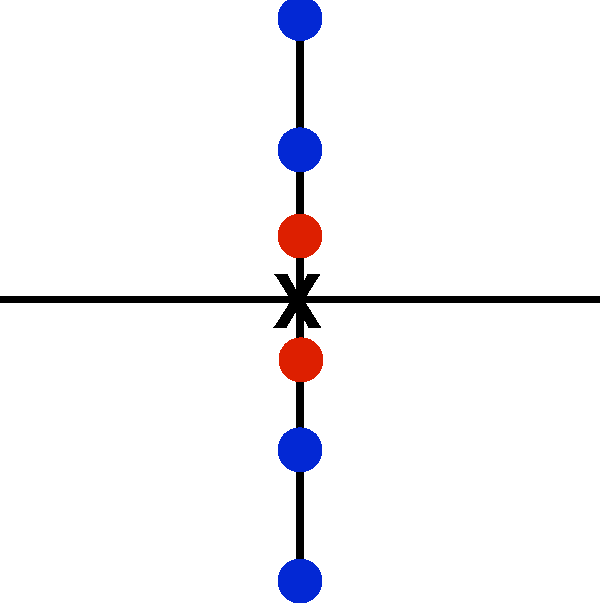
\includegraphics[width=4cm]{periodic/2pulseess}
\end{center}
\caption{Interaction eigenvalues in red, ``essential spectrum'' eigenvalues in blue.}
\end{figure}

We prefer not to restrict ourselves to this case for the following reason. Consider a $2-$periodic pulse with scaling parameter $r$, length parameters $b_0^0 = 1$ and $b_1^0 = \exp(-\pi m_1/\rho)$, and phase parameter $\theta = 0$ (for convenience). If the length parameter $b_1^0$ is sufficiently small (i.e. $m_1$ is sufficiently large), we can \emph{decrease} $b_1^0$ while keeping the same $r$. From Theorem \ref{unifperexist}, we get a whole family of $2-$periodic pulses this way. The domain length is $2X$, where
\[
X \approx C \Big( 2 |\log r| + |\log(b_0 b_1)| \Big)
\]
If we keep $r$ fixed and decrease $b_1^0$ (which decreases $b_1$), $X$ will grow, but the interaction eigenvalues will not change much. On the other hand, the ``essential spectrum'' eigenvalues will move towards the origin. This will cause an ``essential spectrum'' eigenvalue to pass through an interaction eigenvalue. It is unclear at present what happens when these eigenvalues cross, but we have observed Krein bubbles numerically. The $\epsilon-$ball condition gives us an upper bound on the size of these Krein bubbles.

With this out of the way, we can use the following theorem to locate the eigenvalues of \eqref{PDEeig} near the origin.

% eigenvalue location theorem

\begin{theorem}\label{locateeigtheorem}
Assume Hypotheses \ref{Eprimehyp}, \ref{Hhyp}, \ref{hypeqhyp}, \ref{Qexistshyp}, \ref{nondegenhyp}, \ref{c0nonzero}, \ref{Melnikov2hyp}, and \ref{Adistincteigs}. Let $q_{np}(x)$ be a periodic $n-$pulse solution constructed according to Theorem \ref{perexist} with scaling parameter $r \leq r_0$. Let $\delta > 0$ be defined as in Theorem \ref{blockmatrixtheorem}. Then the following are true.

\begin{enumerate}[(i)]

\item There is an eigenvalue at 0 with (at minimum) geometric multiplicity 2 and algebraic multiplicity 3. The eigenfunctions are the kernel eigenfunction $\partial_x q_{np}(x)$ from translation invariance; its generalized kernel eigenfunction $t_{np}(x)$; and a third kernel eigenfunction $v^c(x)$ which is bounded but does not decay exponentially.

\item There exists $r_1 \leq r_0$ such that for every $r \leq r_1$ for which the $\epsilon-$ball condition is satisfied, there are $n - 1$ pairs of interaction eigenvalues given by $\lambda = \pm \lambda^{\text{int}}_j(r)$ for $j = 1, \dots, n-1$, where
\begin{align*}
\lambda^{\text{int}}_j(r) = r^{1/2} \sqrt{\tilde{\mu}_j / M} + \mathcal{O}(r^{3/4})
\end{align*}
These interaction eigenvalue pairs are either real or purely imaginary, and the remainder term cannot move them off of the real or imaginary axis.

\item There exists $r_2 \leq r_1$ such that for every $r \leq r_2$ for which the $\epsilon-$ball condition is satisfied, there are pairs of purely imaginary ``essential spectrum'' eigenvalues given by $\lambda = \pm \lambda^{ess}(X,k; r)$ for every positive integer $k$ with $\frac{c_0 \pi k}{X} < \delta$ (approximately $k < \delta n |\log r|$), where
\begin{equation}\label{lambdaess}
\lambda^{ess}(X, k; r) = c_0 \frac{k \pi i }{X} \left( 1 + \mathcal{O}\left( \frac{1}{X} \right)\right) + \mathcal{O}\left( \frac{r^{1/2}}{X} \right)
\end{equation}
In terms of $r$ and the $b_j$, these are located at approximately
\begin{equation}\label{lambdaessr}
\lambda^{ess}(k; r) = C \frac{k \pi i }{n |\log r| + |\log b_0 b_1 \cdots b_{n-1}|}  \left( 1 + \mathcal{O}\left( \frac{1}{n |\log r|} \right)\right) + \mathcal{O}\left( \frac{r^{1/2}}{n |\log r|} \right)
\end{equation}
The remainder terms cannot move these off of the imaginary axis.

\item For sufficiently small $r$, we have the following two eigenvalue counts.
\begin{itemize}
	\item There exists a small radius $\xi$ (which excludes the interaction eigenvalues and ``essential spectrum'' eigenvalues) such that there are exactly 3 eigenvalues inside the circle of radius $\xi$ in the complex plane. These must be the three eigenvalues from part (i).

	\item There are exactly $2n + 2 k_M + 1$ eigenvalues inside the circle of radius $\tilde{\delta}$ (which may be slightly smaller than $\delta$) in the complex plane, where $k_M$ is the largest positive integer $k$ such that $\lambda^K(k,X) < \tilde{\delta}$. Thus, if the $\epsilon-$ball condition is satisfied, there are no eigenvalues inside the circle of radius $\tilde{\delta}$ other than the ones already accounted for.
\end{itemize}
\end{enumerate}
\end{theorem}

If we can take one of the baseline length parameters $b_j^0$ to be small compared to the others, we are ``close to'' the situation on the real line. Since we are on a periodic domain, we can without loss of generality take $b_{n-1}^0$ to be small. Recall that the other baseline length parameters are given by
\begin{align*}
b_j^0 &= e^{-\frac{1}{\rho}m_j \pi} && j = 0, \dots, n-2
\end{align*}
for nonnegative integers $m_j$. In this case, the parity of the  integers $m_k$ determines the eigenvalue pattern.

\begin{theorem}\label{inteigsparity}
Assume Hypotheses \ref{Eprimehyp}, \ref{Hhyp}, \ref{hypeqhyp}, \ref{Qexistshyp}, \ref{nondegenhyp}, \ref{c0nonzero}, \ref{Melnikov2hyp}, and \ref{Adistincteigs}. Let $r_1$ and $b^*$ be as in Theorem \ref{unifperexist}. Choose an integer $n \geq 2$ and a sequence of $n-1$ baseline length parameters $b_0^0, \dots, b_{n-2}^0$, where $b_j^0 = \exp\left(-\frac{1}{\rho}m_j \pi\right) \in \mathcal{B}$. 

Then there exists $\tilde{r_1} \leq r_1$ and $\tilde{b}^* \in \mathcal{B}$ with $\tilde{b}^* \leq b^*$ such that for any $r \leq \tilde{r}_1$, $b_{n-1}^0 \in \mathcal{B}$ with $b_{n-1}^0 \leq \tilde{b}^*$, and $\theta \in [-\arctan \rho, \pi - \arctan \rho)$, we have the following result.

Let $r = \exp\left( -\frac{1}{\rho} m \pi \right)$, where $m$ is a nonnegative integer. If $M > 0$, then 
\begin{itemize}
\item If $m$ is even ($m$ is odd), there are $n_{\text{even}}$ purely imaginary (real) pairs of interaction eigenvalues.
\item If $m$ is even ($m$ is odd), there are $n_{\text{odd}}$ real (purely imaginary) pairs of interaction eigenvalues.
\end{itemize}
where $n_{\text{even}}$ is the number of even $m_0, \dots, m_{n-2}$ and $n_{\text{odd}}$ is the number of odd $m_0, \dots, m_{n-2}$. If $M < 0$, these are reversed.
\end{theorem}

Finally, we consider the case of the 2-periodic pulse. For the symmetric 2-periodic pulse (i.e. $b_0 = b_1$), the interaction eigenvalues are approximately

\[
\lambda^{\text{int}} = \pm C r^{1/2} e^{-\theta/2\rho} \sqrt{ \frac{1}{M} \left( \rho \cos \theta - \sin \theta \right) }
\]

which is 0 at $\theta = \arctan \rho$. At a point near there, there is a bifurcation in which a pair of real eigenvalues collides at 0 and then becomes a pair of purely imaginary eigenvalues. We can probably use a symmetry argument or something like that to show that this occurs for small $r$ at the actual pitchfork bifurcation point $\theta^*(r)$, where $\theta^*(0) = \arctan \rho$. This has been verified numerically.

\iffulldocument\else
	\bibliographystyle{amsalpha}
	\bibliography{thesis.bib}
\fi

\end{document}